%author: yjw, 2024-4-1

在 ROS 2的体系结构中,节点(Node)是最基本的执行单位,负责特定功能的实现,如数据处理或硬件接口。
每个节点可以包含多种通信机制,包括订阅者(Topic Subscribers)、定时器(Timer)、服务服务器(Service Servers)
和服务客户端(Service Clients),如图\ref{pic:rns}。这些通信实体的目的是为了接收和发送数据,以及提供不同的服务。

节点注册到执行器(Executor)中,执行器是一个控制实体,负责协调节点的活动。
当节点的一个通信事件发生时,比如收到一个主题消息或服务请求,执行器会调用相应的处理函数,或称为回调函数(Callback)。
这些回调函数是预先定义的,用来响应特定类型的事件,如 \texttt{topic\_receive()} 用于处理主题消息,
\texttt{request\_receive()}用于处理服务请求,\texttt{time\_up()}用于处理定时器完成计时。

在节点的生命周期中,可以使用生命周期状态机(Lifecycle SM)来管理节点的状态,这在管理复杂节点时特别有用。
生命周期状态机允许节点在不同状态之间转换,如激活(activate)、去激活(deactivate)和清理(cleanup)。
每个状态变化都可以有对应的回调函数,例如\texttt{setting()}在节点激活时调用,用于声明节点接口、
节点执行器(Executor)、通信订阅和服务订阅等一系列节点功能实体;\texttt{activate()} 用于节点初始化完毕开始服务,
此时节点处于正常工作状态; \texttt{cleanup()}在节点清理资源时调用,用于释放节点所持有的微机资源。

\textbf{ROS事件处理机制}: 

节点调用 \texttt{spin()} 函数来持续检查和处理事件,如伪代码\ref{lst:ros_spin}。

\begin{lstlisting}[language=Python, caption=ROS2事件循环示例, label=lst:ros_spin]
spin():
    while True:
        new_msg <- ros_dds_listener()
        handler <- get_callback(new_msg)
        Executor.execute(*handler)
        sleep(0.1)
\end{lstlisting}

\texttt{spin()} 实质是一种事件循环,它会保持节点循环和监听,检查系统中是否有新的ROS消息或待处理的消息,获取到消息实体后,
根据消息类型获取节点初始化时注册的回调函数,交付给节点执行器去执行,从而完成对该事件(消息)的响应。
\texttt{spin()}函数是一个事件循环,保持节点持续运行并响应事件。

在执行器内部,\texttt{execute\_any\_*()} 函数是对ROS核心细节的抽象,这个函数根据事件的类型和优先级选择一个
事件来处理。处理过程包括执行注册的回调函数,这些函数是在节点初始化时注册的,如\texttt{timer.registe\_handler()} 
用于注册定时器事件的回调;\texttt{subscriber.regeste\_handler()} 用来注册监听到某话题时触发的回调函数,以处理该数据。

总体而言,ROS2的程序机制基于事件驱动的模型,通过节点、执行器和回调函数协同工作来响应和处理各种事件,
这些事件可能来源于数据的接收、定时器的触发、服务的请求和响应,以及节点生命周期状态的变化。
通过这种灵活且模块化的设计,ROS 2能够支持复杂且多样化的机器人系统开发。


\begin{figure}[h]
    \centering
    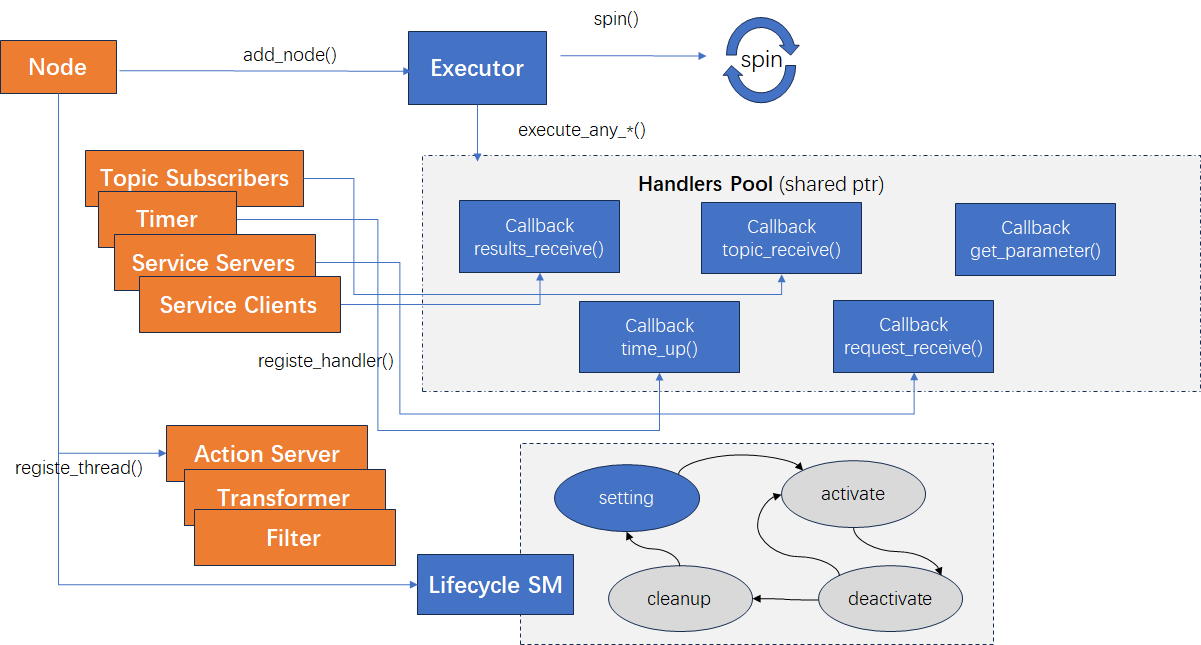
\includegraphics[width=15cm]{ros_node_setup.png}
    \caption{ROS节点内部模型, 初始阶段}
    \label{pic:rns}
\end{figure}

\textbf{ROS 节点释放}

当ROS2系统的节点将释放时,节点的生命周期状态机会从 activate 状态转换为 deactivate 状态,
此状态仅用于让节点完成必要的最后工作,如完成正在处理的数据传输或请求,然后进入非活跃状态。

紧接着,节点生命周期状态机转为 cleanup 状态,见图\ref{pic:rnc},调用 \texttt{cleanup()} 回调函数来释放节点
拥有的资源,这包括所有回调函数(callback handlers),如和话题订阅、定时器、服务等回调
函数。然后清理节点所打开的文件,断开网络连接,释放ROS2上下文,最终释放内存。

\begin{figure}[h]
    \centering
    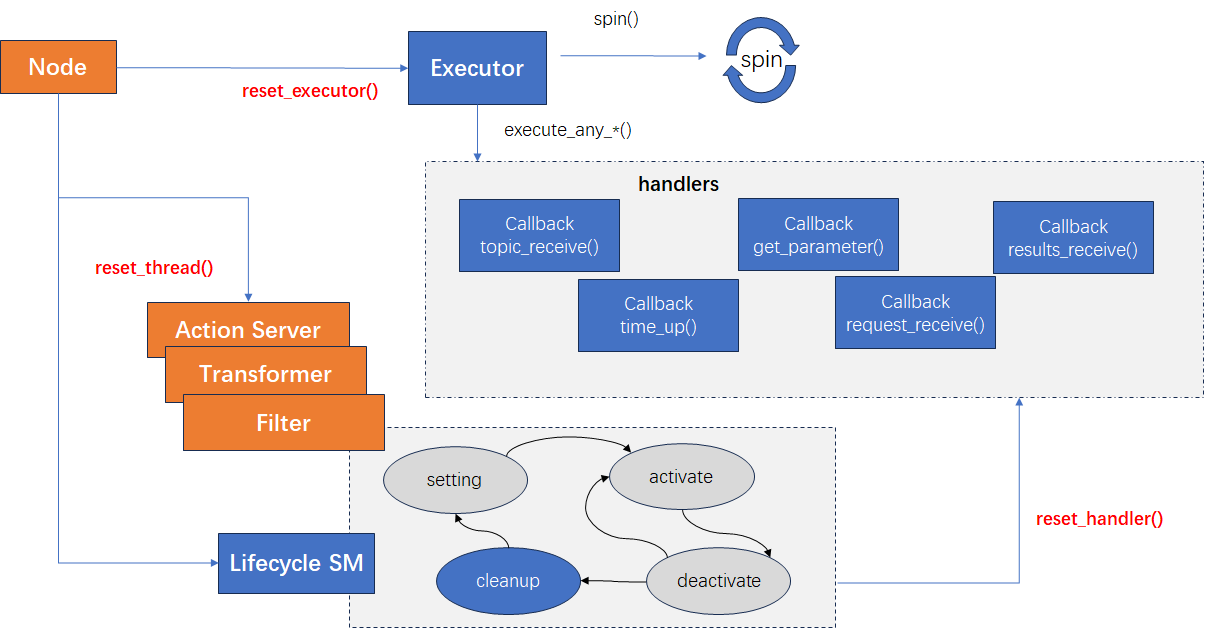
\includegraphics[width=15cm]{ros_node_cleanup.png}
    \caption{ROS节点内部模型, 释放阶段}
    \label{pic:rnc}
\end{figure}

\textbf{ROS 通信机制}

为了适应机器人系统中复杂的通信需求,ROS2设计了一套专用的通信模型。其基础为“发布、订阅“模型,支持节点间的异步数据交换。
该机制允许ROS2系统内的节点(Node)独立地发布(Publish)和订阅(Subscribe)消息,而不需要彼此之间的直接连接或相互了解。
这种设计显著提高了系统的灵活性和扩展性,因为它允许任何数量的发布者和订阅者存在于同一个话题上,从而实现了高效的多对多通信。

在ROS 2的架构中,每个节点可以根据其功能需求,声明为发布者或订阅者,类似图 \ref{pic:rmp},或同时充当这两种角色。
发布者负责生成并发布特定类型的消息到一个命名的话题上,而订阅者则监听这个话题,接收并处理传入的消息。
监听到并处理消息时,使用的是订阅该话题时传入的回调函数来自动处理,订阅者不必同步阻塞就能等待处理订阅消息。
话题本质上是一个数据通道,它通过唯一的名称标识,确保消息的传递和接收的一致性。
每个话题都与一个明确的消息类型相关联,这个消息类型使用YAML格式定义各字段的静态变量类型,从而定义了该话题传输数据的结构。

此通信机制的一个核心优点是其异步性,使得发布者和订阅者可以独立地操作,增加了处理并发消息的能力。
此外,由于发布者和订阅者之间的解耦,系统组件可以被设计得更为模块化,易于开发和维护。
例如,在自动驾驶的应用场景中,激光雷达传感器节点可以发布其测量到的数据到话题 \textbackslash scan,而负责建图和规划路径的节点
则通过订阅该话题来实时获取雷达信息,从而完成最终决策。


\begin{figure}[h]
    \centering
    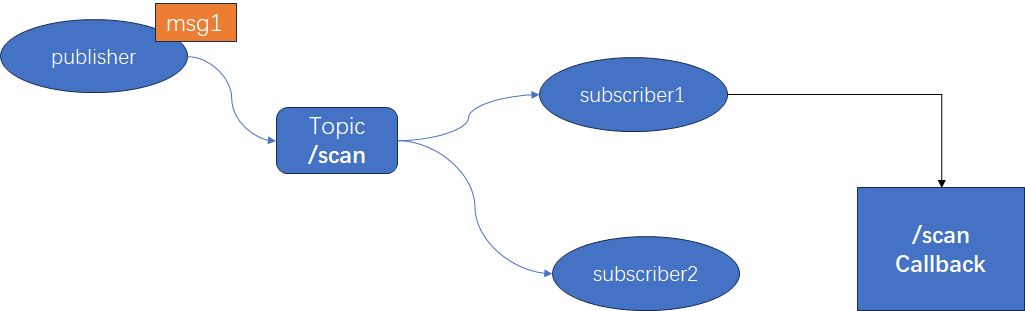
\includegraphics[width=13cm]{ros_msg_passing.png}
    \caption{ROS话题通信机制}
    \label{pic:rmp}
\end{figure}